\documentclass[10pt]{article}
\usepackage[usenames]{color} %used for font color
\usepackage{amssymb} %maths
\usepackage{amsmath} %maths
\usepackage[utf8]{inputenc} %useful to type directly diacritic characters

\usepackage{tikz-feynman}
\begin{document}
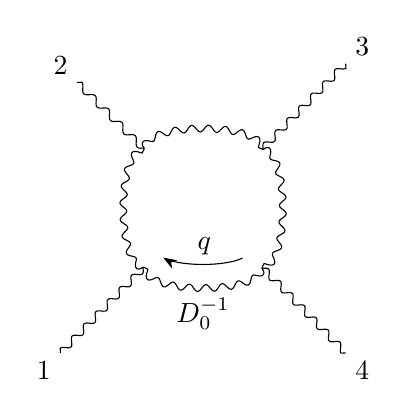
\begin{tikzpicture}
\begin{feynman}
  \vertex (k2) {2};
  \vertex [below right=of k2] (c);
  \vertex [right=of c] (d);
  \vertex [above right=of d] (k3) {3};
  \vertex [below=of c] (b);
  \vertex [right=of b] (a);
  \vertex [below left = of b] (k1) {1};
  \vertex [below right = of a] (k4) {4};
  
  \diagram* {
    (a) -- [boson] (k4),
    (b) -- [boson] (k1),
    (c) -- [boson] (k2),
    (d) -- [boson] (k3),
    (a) -- [boson, half left, looseness=0.6, momentum'=\(q\), edge label=\(D_0^{-1}\)] (b),
    (b) -- [boson, half left, looseness=0.6] (c),
    (c) -- [boson, half left, looseness=0.6] (d),
    (d) -- [boson, half left, looseness=0.6] (a),
  };
\end{feynman}
\end{tikzpicture}


\end{document}